\documentclass[../../main.tex]{subfiles}
\begin{document}

\subsection*{10.15}
Una bobina circolare compatta, formata da $N_1 = 3 * 10^3$ spire di raggio $R = 25\ cm$ è collegata ad un misuratore di f.e.m.; una seconda bobina compatta coassiale alla prima e ad essa parallela, composta da $N_2 = 100$ spire di raggio $r = 0.5\ cm$, è percorsa dalla corrente $i = 15\ A$ e si muove lungo l'asse x con velocità costante.\\
Calcolare il coefficiente di mutua induzione M(x) in funzione della distanza x tra i centri e il valore $\varepsilon(x)$ misurato nella prima bobina quando la seconda ha velocità $v = 20\ \frac{m}{s}$.\\
Assunto $x = 0.1\ m$ calcolare la corrente che fluisce nella prima bobina assunta la sua resistenza uguale a $R  = 2\Omega$ e la forza esercitata su di essa.\\
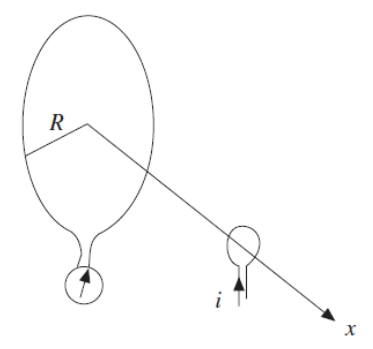
\includegraphics[scale=0.3]{e_10_15.png}
\subsubsection*{Formule utilizzate}
\subsubsection*{Soluzione punto a}

\subsubsection*{Soluzione punto b}
\newpage

\end{document}